\documentclass[twoside,a4paper]{article}
\usepackage{geometry}
\usepackage{booktabs}
\usepackage{tabu}
%for some reason the compiler kills itself with {comment} package
\newgeometry{
  top=0.75in,
  bottom=0.75in,
  outer=1in,
  inner=1in,
}
\usepackage{graphicx}
\usepackage{amsmath}
\usepackage{siunitx}
\usepackage{cancel}
\usepackage{float}
\usepackage{subcaption}
\usepackage[
backend=biber,
style=numeric,
sorting=none
]{biblatex}
\usepackage[T1]{fontenc}
\usepackage[utf8]{inputenc}
\usepackage[english]{babel}

\addbibresource{mybibliography.bib}
\title{\textbf{FIT Report} \\[1ex] \large Report 1 \\[2ex] \Large \underline{Handwriting detection and Note Conversion using OCR}}

\author{Piętka Ł, Barot H, Krzysztosiak M, Markowicz J, Milewski M, Sobczak M}
\date{March 12 2025}
\begin{document}

\maketitle
\tableofcontents
\newpage
\section{Introduction}
The aim of this project is to create a tool for digitizing handwritten notes written in the English language into readable text in ASCII format. The tools utilized in this project are existing OCR models along with various preprocessing techniques applied to training data in order to minimize computational time and discard unnecessary information. \\\\
We feel the applicability of such a tool is rather high as it would allow for a streamlined process of digital note making and sharing for those who prefer a traditional method of note keeping. In addition, such a tool could be utilized to increase the efficiency of tutors in correcting the test papers of their students.

\subsection{Background Knowledge}
This project focuses primarily on the use of Optical Character Recognition (OCR) models to convert handwritten text into digital text. 
OCR is a technology that is used to convert different types of documents, such as scanned paper documents, PDF files, or images captured by a digital camera, into text files that can be easily edited, searched, and stored on a computer.\\


%i think its better to keep the background knowledge short, he said to just give the term and a citation for stuff instead of explanations. 
%OCR is a technology that is used to convert different types of documents, such as scanned paper documents, PDF files, or images captured by a digital camera, into editable and searchable data. The OCR technology is used to convert virtually any type of image containing written text (typed, handwritten, or printed) into machine-readable text data. \\


\subsection{Problem Statement}
The main problem that this project aims to solve is the inefficiency of converting handwritten notes to digital text. 
This is a common problem for students, teachers, and professionals who prefer to take notes by hand. 
The process of converting handwritten notes into digital text is time-consuming and error-prone. 
This project aims to develop a tool that can automate this process and make it more efficient and accurate. \\
 
\section{Methodology and Procedure}
There are various steps involved in the process of converting handwritten notes into digital text using OCR technology, and it is best to break down the problem into smaller problems.
The following steps are involved in the process:
\begin{enumerate}
    \item Data Collection
    \item Data Preprocessing
    \item Model Training
    \item Model Evaluation
    \item Model Deployment
\end{enumerate}

\subsection{Data Collection}

%The first problem is to decide the type of data that will be used to train the OCR model. It is relatively easy to implement an OCR model that recognizes single characters. Since, it's only job is to convert that one specific character.
%But when it comes to whole sentences, pages, and books, the problem becomes more complex. The model still has to recognize single characters, but also their placement relative to other characters.

%Hence, we need a data set that contains images of handwritten text and the corresponding text that is written in the image with it's relative location on the image. 

The first problem we faced was deciding what kind of data we should collect to train the OCR model.\\
The choice of the model should reflect the purpose of our project and, as such, we browsed for information and prepared a comparison between some notable datasets and their characteristics chosen based on our research. (Table 1)


    %There are many existing models on the Internet that are freely available and easy to implement into our project, however we still needed to train it on data that would fit the purpose of our project.
    %feels redundant after i wrote it, feel free to uncomment if you disagree
We decided to use the freely available TrOCR model as it comes pre-trained for simple single-word recognition problems, however, it struggles with handwriting and full documents and thus needed to be fine-tuned.\\
Data found in the real world would differ in many aspects as the equipment used to take the images, the lighting used, and the handwriting of each person may vary, as such, the data should cover different lighting conditions, various handwriting styles, and varied image qualities (within reason). \\
For the training data, we used the GNHK dataset~\cite{Lee2021} which consists of real world examples of handwriting suitable for training and testing of the model. \\
The rationale behind choosing this dataset was simple as the data provided aligns with our goal, allowing us to fine-tune the model for the specific purpose of recognizing handwritten notes.\\
For the testing data, we plan to utilize both the GNHK dataset examples as well as our own handwritten notes.
%i dont know how to add citations, https://www.goodnotes.com/gnhk , ideally this would be a citation in [1].
\newpage
\begin{table}[!ht]
    \centering
    
    \caption{Comparison of Handwritten Text Datasets}
    \renewcommand{\arraystretch}{1.3} % Adjusts row height for better readability
    \begin{tabular}{|p{3cm}|p{5cm}|p{2.5cm}|p{2.5cm}|}
    \hline
        \textbf{Dataset} & \textbf{Characteristics} & \textbf{Training Size} & \textbf{Testing Size} \\ \hline
        CEDAR~\cite{CEDAR_Dataset} & Scans of handwritten letters at 300 DPI, developed in 2002. & 5321 & N/A \\ \hline
        MNIST (Archived)~\cite{MNIST_Dataset} & Grayscale images with normalized sizes, reducing preprocessing time. & 60,000 & 10,000 \\ \hline
        GNHK~\cite{Lee2021} & Camera-captured handwritten notes with 1080p to 4k resolution, lighting, and backgrounds. & 515 & 172 \\ \hline
    \end{tabular}
    \label{tab:datasets}
\end{table}

%\newpage
%\pagebreak
\subsection{Data Preprocessing}

%The preprocessing of the training data as well as real data is a crucial step in the process of converting handwritten notes into digital text as it both narrows down on what the model should be trained for and reduces the computational time.\\
%When normalizing data from different sources within a large data set there are certain variables that need to be controlled.
%Such as brightness levels, the angle of the image, the size of the image, and the quality of the image. Since the end user will not be taking these pictures in ideal and controlled conditions,
%a certain amount of preprocessing is required to make all images have the same features. 
The data collected for training and testing may come from different sources and as such different equipment (in this case a camera or a scanner) may have been used to obtain it, or it may differ in quality standards. Because of that, certain variables need to be controlled through normalization to provide any significant information. The preprocessing of data aims to solve the problem of controlling the quality of data used to fine-tune the model for our purpose, reduce the computational time, and narrow down the information we want to extract from real data.\\
After reading research papers on the subject~\cite{Tensmeyer2015}, we decided on a list of variables that need to be controlled and the corresponding preprocessing approaches:
%[2] relevant literature: https://arxiv.org/pdf/1509.03456
\begin{itemize}
    \item Brightness levels and lighting
    \item Image size
    \item Image resolution
    \item Coloured image should be converted to grayscale
    \item Geometric distortions caused by the angle of the camera
    \item Compression and artifacts.
\end{itemize}
For \textbf{brightness levels} and \textbf{colours}, the images should be converted to grayscale for increased accuracy. Then a transformation called histogram equalization can be performed to normalize the brightness levels.\\
Histogram equalization improves the contrast of an image by spreading out the most frequent intensity values, making the histogram of the output image approximately uniform, for that purpose we utilized the relevant function in the OpenCV library.~\cite{OpenCV_Histogram_Equalization}\\
A thresholding algorithm should also be used to separate the text and the background, including phenomena such as shadows caused by lighting that obscure the text, for this purpose, we utilize Otsu thresholding~\cite{Tensmeyer2015} via the relevant OpenCV function~\cite{OpenCVThresholding}.
%[3] relevant sources: https://arxiv.org/pdf/1509.03456 section 3.4 ; [4] https://docs.opencv.org/4.x/d7/d4d/tutorial_py_thresholding.html
%idk what to write about iamge size and resolution, my take is throw out the data, upscaling seems pointless
%perhaps we can add some images to show as examples of the preprocessing we use or maybe a block diagram of the process like in the paper
\\
For \textbf{image size} and \textbf{resolution}, it is important to ensure that all images fed into the model are of a consistent size and resolution. This helps in maintaining uniformity and reduces the complexity of the model. Images that are too small may not contain enough detail for accurate recognition, while images that are too large may introduce unnecessary computational overhead. Therefore, resizing the images to a standard resolution is a crucial preprocessing step. We used OpenCV to upscale all images to a consistent resolution.
\\
For \textbf{geometric distortions}, images may be taken at various angles, leading to distortions that can affect the accuracy of the OCR model. To correct these distortions, we applied geometric transformations such as rotation and perspective correction. These transformations help to align the text properly, making it easier for the OCR model to recognize the characters accurately. OpenCV provides functions for these transformations, which we utilized to preprocess the images.
\\
For \textbf{compression and artifacts}, images can suffer from compression artifacts, especially if they are saved in lossy formats like JPEG. These artifacts can introduce noise and reduce the quality of the image. To mitigate this, we saved all images in a lossless format like PNG during preprocessing to avoid creating more artifacts. Additionally, we applied denoising techniques using OpenCV to remove any existing artifacts and enhance the quality of the images.


\subsection{Limitations}
In addition to all the tools and techniques utilized, we feel it is important to note the limitations of the assumptions and data collection.\\
The project assumes that images will be taken with the quality that is within reason, as such images should be taken with the intent of being legible, and thus input data with significant resolution problems, or pitch dark lighting ought to be ignored as they are not representative of the problem we aim to solve.\\
The dataset we used presents a vast amount of images differing in quality and handwriting styles, however, we understand that more sources could be utilized.\\


\newpage
\begin{center}
  \textbf{\Large Report 2}
\end{center}

\section{Re-evaluating: Report 1}

In report 1, the aim of the project was stated to be creation of  a program that utilizes OCR technology, which allows for recognition and digitization of handwritten notes 
into easily readable and storable text documents on a computer. However, the project was not clearly defined and the problem statement was not well articulated.
The target population was not specified, and the aim of the project was not clearly defined. The project lacked a clear focus and direction, which made it difficult to understand the purpose and goals of the project.

Due to the target population being vague, multiple areas of this project were hard to define, and ambiguous as to what direction the project is headin in.
This was a major roadblock because when we discussed questions like "Do the samples include math equations?" or "Do the samples include letters?" "Are the letters allowed to be geometrically malformed or the the samples have to be
clean and perfectly written?". Our group memmbers had different approaches to these questions, and this led to a lot of confusion and miscommunication.

Hence, this report would like to revisit and address the flawed initial approach. Define the who the project is for, which will make it simpler to find source of raw data,
and implement a model that will best suit the use case defined.

\subsection{Problem Statement}
Certain two members of our group particularly enjoyed writting english literature. Wether it was analitical essays, or fantasy stories. They both agreed that writting on a physical paper felt the most comfortable and natural. However, they couldn't organize their raw notes and digitizing them was 
really time consuming. Hence, we decided to create a program that would help them with this problem. The specific aim of this project is to create a program
for the the two members of our group, that could assist in digitization of their english literature notes.

\section{Data Collection Procedure: }
In the previous report, we decided to use the GNHK dataset~\cite{Lee2021}, as it best suited the freely available OCR model that we chose. However, this was a large dataset, that contained
a variety of different samples. The sample types included math equations, plain english text, distorted handwritting and much more. Additionally these datasets conainted a the different types of english (british, american, asian) used all over the world.

This essentially ment, that this dataset ranged over a wider domain than what was needed for our project. This is displayed using 
a venn diagram in figure~\ref{fig:venn_diagram}. Set A (red circle) is the collectioon of what GNHK has to offer, meanwhile Set B (blue circle) is
what is required for our project. The intersection of the two sets is what we need.
\begin{figure}[H]
  \centering
  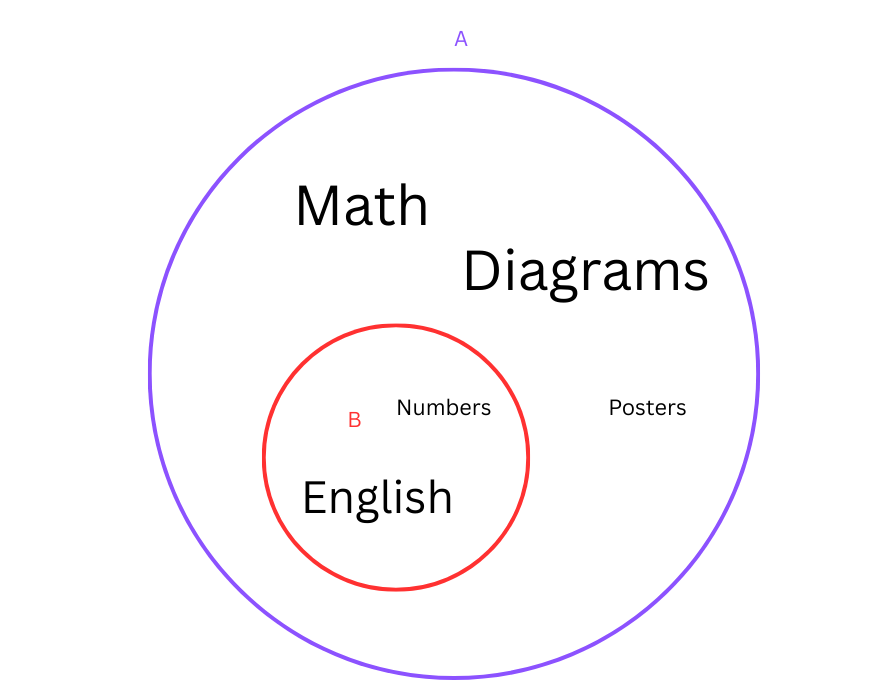
\includegraphics[width=0.8\textwidth]{VennDiagram_WhatWeNeed.png}
  \caption{Venn Diagram of Dataset Characteristics vs. Project Needs}
  \label{fig:venn_diagram}
\end{figure}

To collect the data we had two choices: 
\begin{enumerate}
  \item We could have used the GNHK dataset, and filtered out the samples that we did not need. However, this would be a time consuming process, and we would have to manually go through each sample.
  \item The target population (two writters) are asked to send samples of their handwritting, of this exact same sentence. 
\end{enumerate}

We decided to go with the second option, as it would be much easier to collect and it would be more represntative of the target population's needs.
The sentence chosen was "The quick brown fox jumps over the lazy dog". This sentence was chosen because it contains all the letters of the english alphabet, and it is a common pangram used in handwriting samples.
Additionally, the users were asked to write this sentence in all lowercase or uppercase, alternating between them. They were also asked to number each line, to get alphanumeric data.


\section{Raw Data (samples and syntactic characteristics): }
As the method collection procedure was described in the previous section, the raw data was collected from the end target users.
Here is a sample image from the data from both users:
\begin{figure}[H]
  \centering

  \begin{subfigure}[b]{0.45\textwidth}
    \centering
    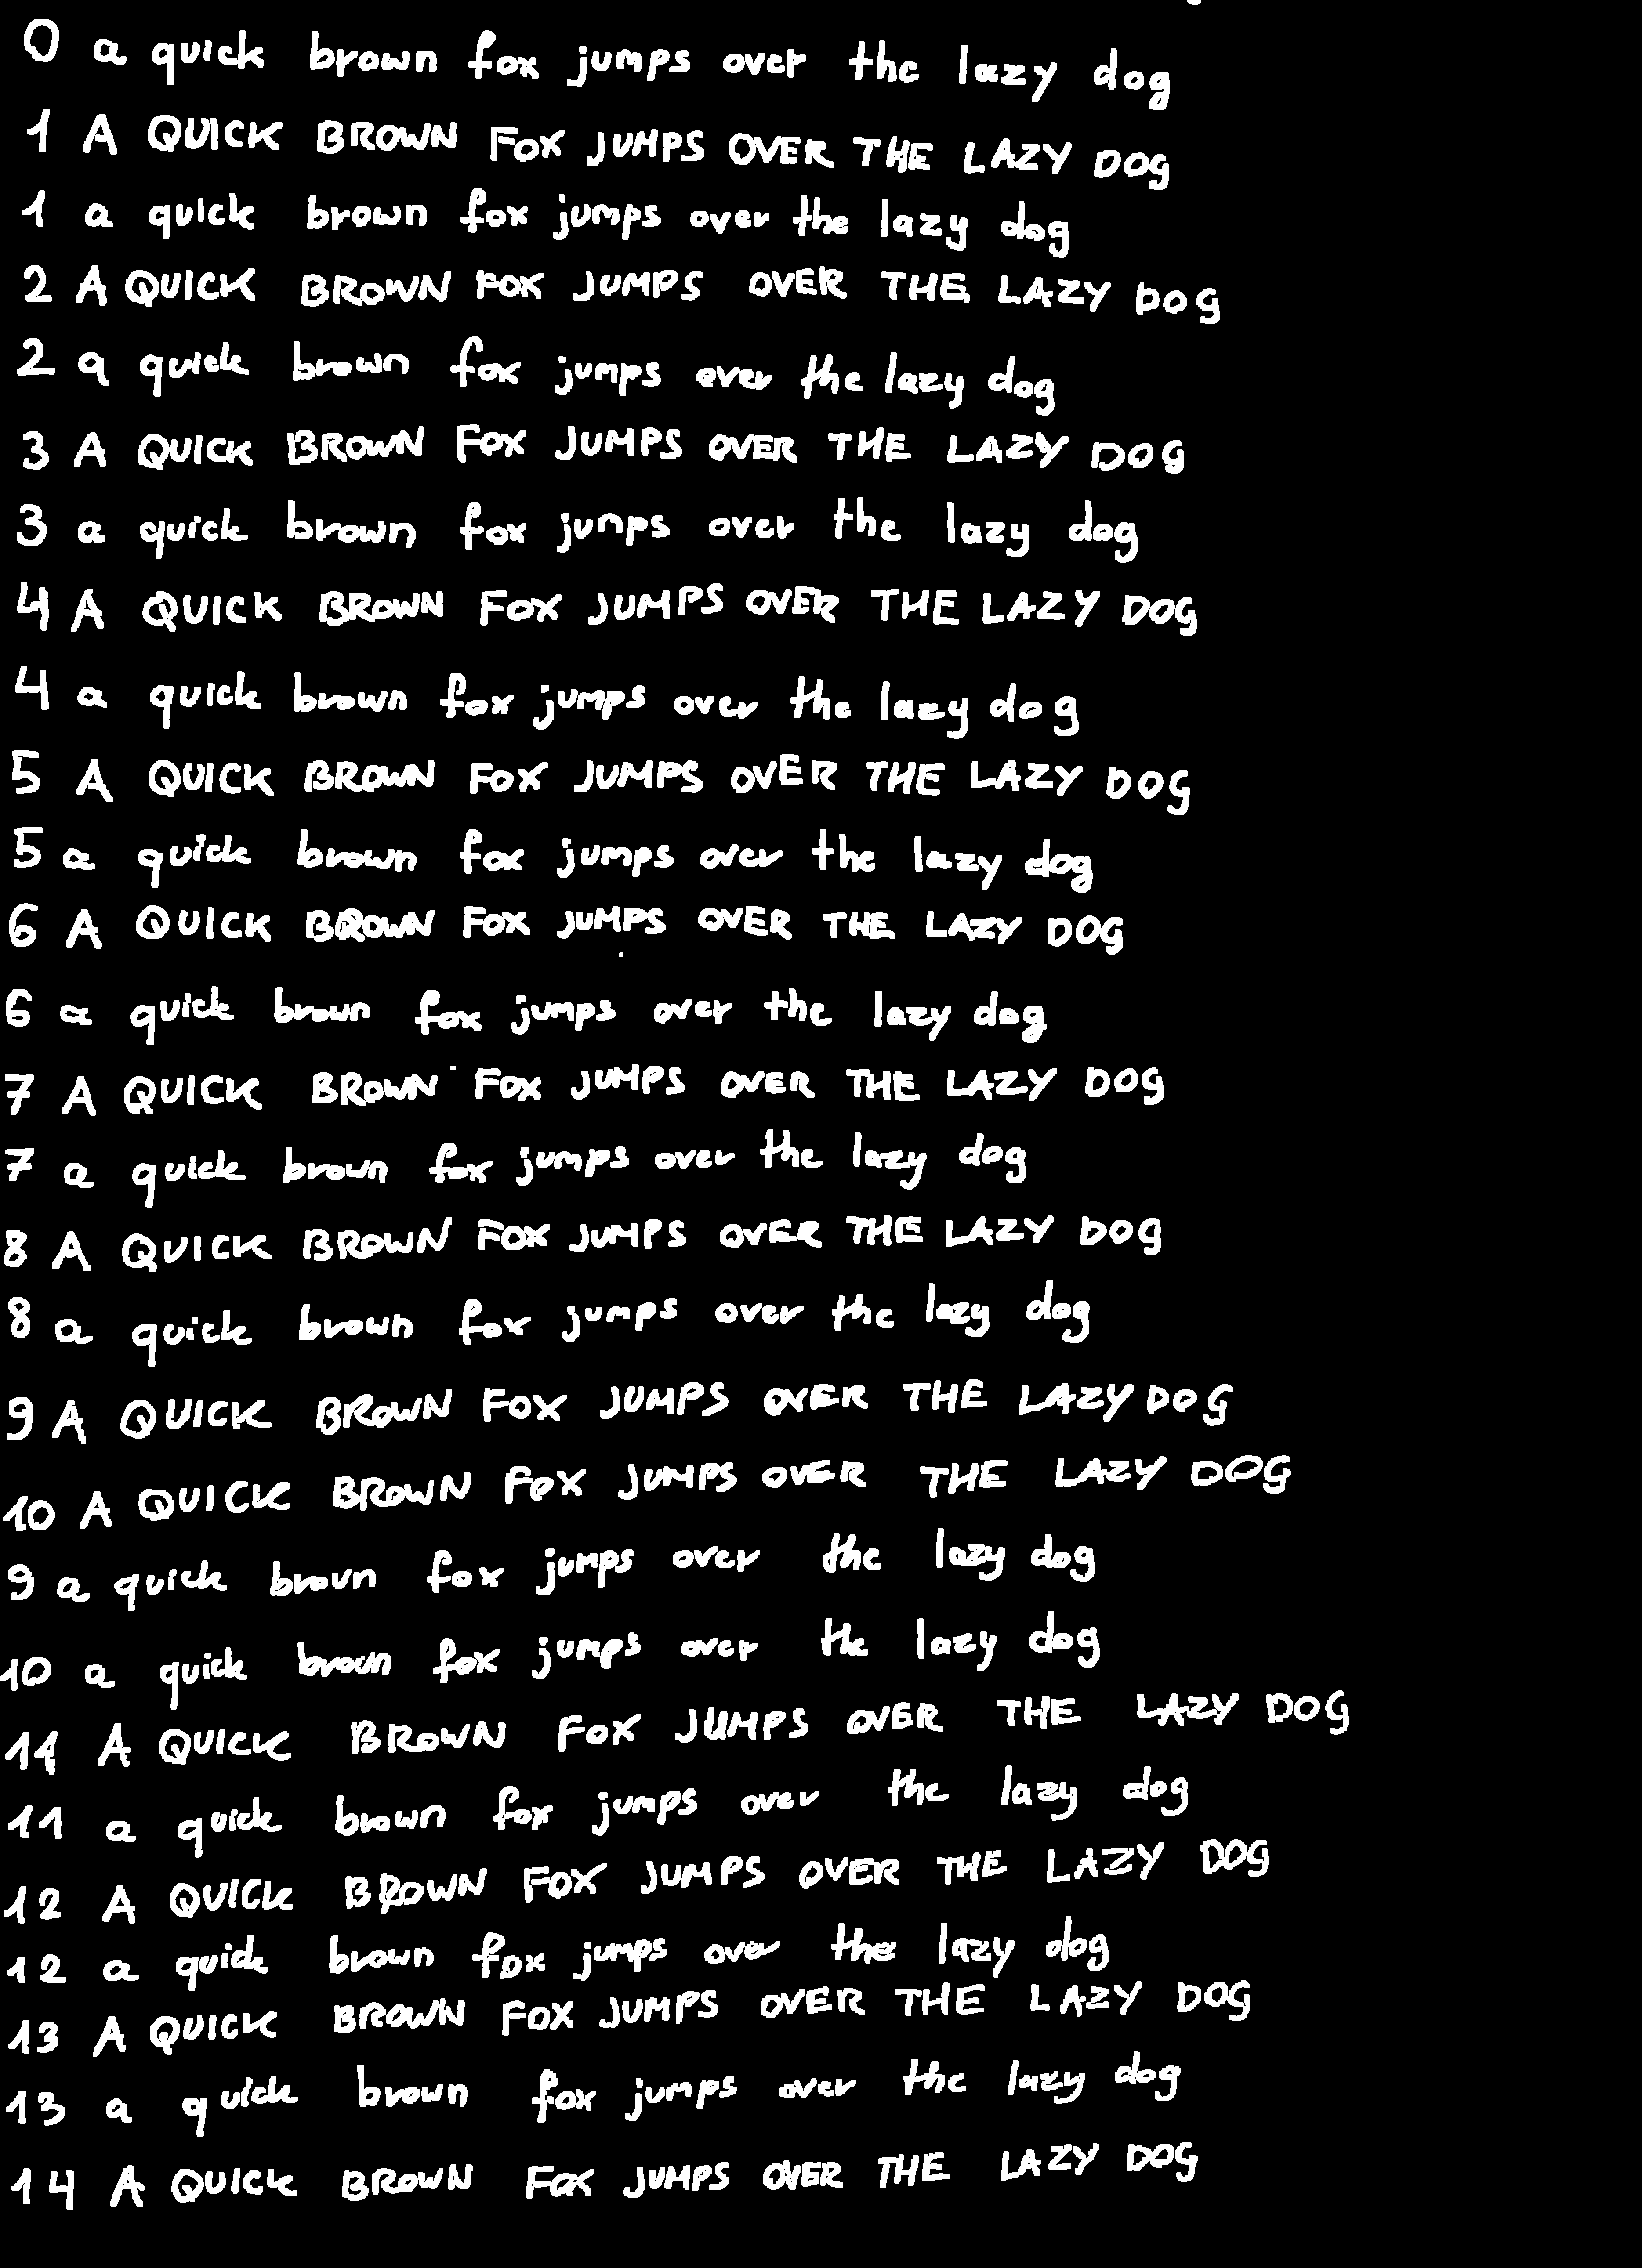
\includegraphics[width=\textwidth]{L1.png}
    \caption{User 1 -submitted handwriting }
    \label{fig:l1_sample}
  \end{subfigure}
  \hfill
  \begin{subfigure}[b]{0.45\textwidth}
    \centering
    \includegraphics[width=\textwidth]{kuba1.jpg}
    \caption{User 2 -submitted handwriting }
    \label{fig:kuba_sample}
  \end{subfigure}

  \caption{Side-by-side comparison of dataset and user handwriting samples}
  \label{fig:raw_data_sample}
\end{figure}
The comparison of the two samples as shown in figure~\ref{fig:raw_data_sample} shows that, there are some similarities between the two users writting styles
such as the letter ``q'' and ``Q'', are close to identical between the two user. Despite the similarities, there are also some differences between the two users, such as the letter ``f'' , which are different between the two users.
\\
This is important to note, as a decision must be made on to train two separate models for each user, or to train one model that recognises both handwritting styles.
To understand which choice is more beneficial, we need to understand how we aim to make our model work. First and foremost, a sample must be normalized. This is done to get rid of geometric deformations,
shadows, background. The normalization aims to create a binary image, where 0 means the background, and 1 means the text. This is done using a combination of histogram equalization and thresholding.

After the normalization is done, the image is split into individual letters. This helps creating a dataset of letters, with 61 classes (26 lowercase, 26 uppercase, 10 digits).

After the processing is done, we are left with a very normalized data. This leads to the question weather it is efficient to train different models for each user, or not. 
We believe training two models is feasible, as once the final product runs, a user can "log into" his profile, and have a personalized model. This will increase the accuracy of both models.

However, for the sake of this project, we will train one model, on the name of user 1, and if that will be a seamless process, we will retrain it on mixed data. 


\section{Normalization of Raw Data: }
Lets choose User 1 as an example of Normalization. In report 1, number of image processing techniques were mentioned, such as histogram equalization,
thresholding, resizing, and denoising. But firstly we need to start with smoothening of the image. There are three smoothening filers.
\begin{itemize}
  \item \textbf{Gaussian filter}: Greate for general noise reduction
  \item \textbf{Median filter}: Attempts to preseves edges, while removing noise
  \item \textbf{Bilateral filter}: Provides a balance between smoothening and edge preservation.
\end{itemize}
\begin{figure}[H]
  \centering
  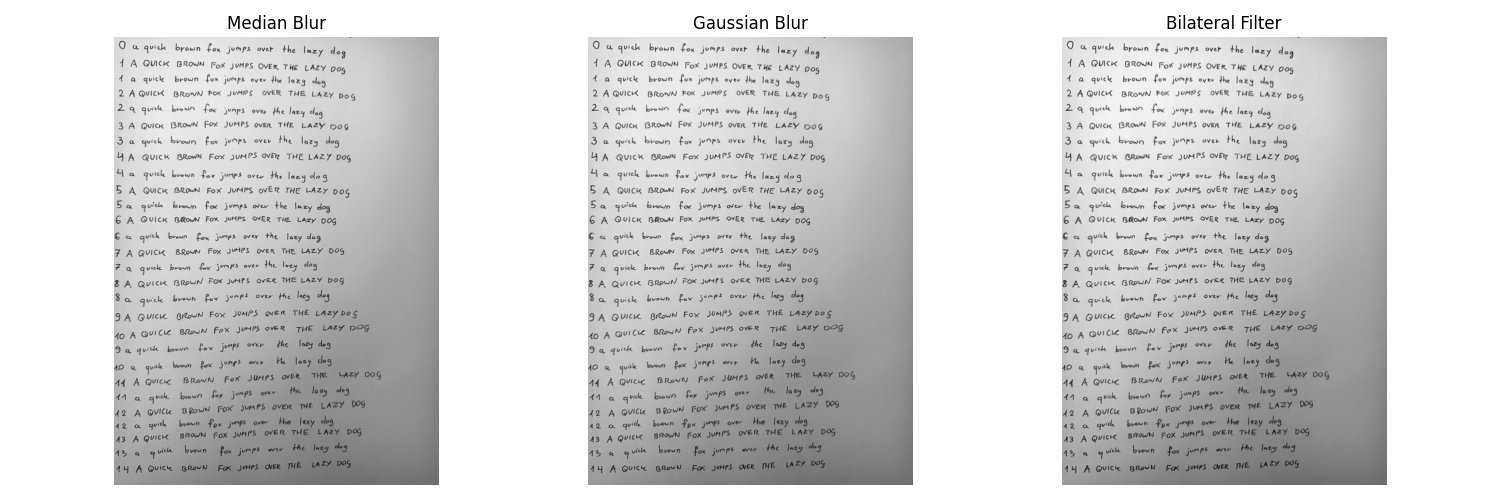
\includegraphics[width=0.8\textwidth]{Comparison_Blues.png}
  \caption{Comparision of three Smoothening filters applied to the same image}
  \label{fig:smoothening_filters}
\end{figure}
The figure~\ref{fig:smoothening_filters} shows the comparison of the three filters. Although all of them look near identical when applied to the image, a subjective view on the comparison is that median blur makes the image darker, but lighting more balanced, than the other 2.
Due to this reason, we decided to use the median filter for our project.\\
\\
Moving onto thresholding, again we consider three different methods:
\begin{itemize}
  \item \textbf{Otsu's method}: Minimizes intra-class variance. Good for images where there is clear distinction between foreground and background.
  \item \textbf{Adaptive Mean thresholding}: Averages neighbouring pixels and subtracts a constant value. Great for varying lighting conditions.
  \item \textbf{Gaussion thresholding}: Similar to adaptive mean, but uses a Gaussian weighted average. Great for images with not too dynamic lighting.
\end{itemize}
\begin{figure}[H]
  \centering
  \includegraphics[width=0.8\textwidth]{Comparison_Thresholding.png}
  \caption{Comparision of three Thresholding methods applied to the same image}
  \label{fig:thresholding_filters}
\end{figure}


\section{Extraction of words/letters: }
\section{Closing Thoughs: }
\printbibliography
\end{document}